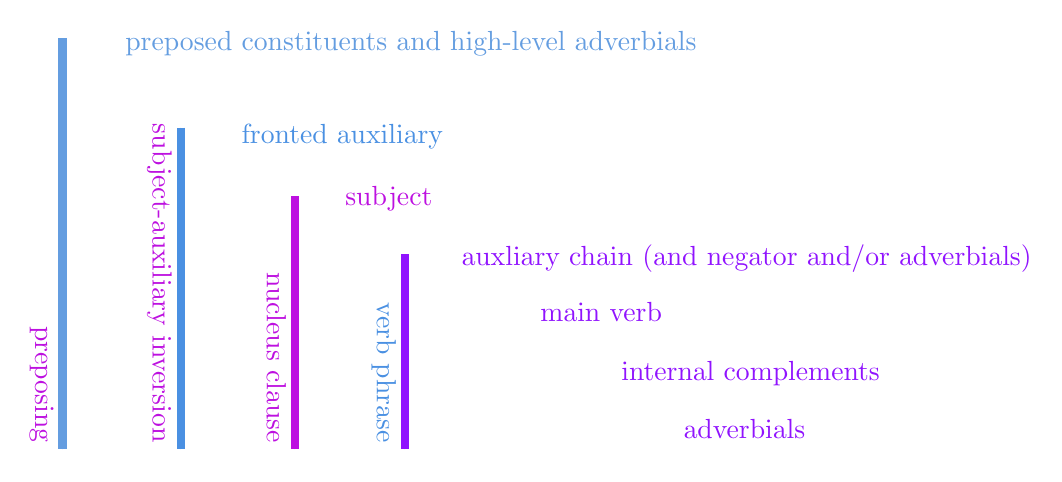
\begin{tikzpicture}[x=0.75pt,y=0.75pt,yscale=-1,xscale=1]
    %uncomment if require: \path (0,300); %set diagram left start at 0, and has height of 300
    
    %Straight Lines [id:da48517433952426825] 
    \draw [color={rgb, 255:red, 144; green, 19; blue, 254 }  ,draw opacity=1 ][fill={rgb, 255:red, 144; green, 19; blue, 254 }  ,fill opacity=1 ][line width=3]    (368,138.93) -- (368,232.93) ;
    %Straight Lines [id:da4265308922026523] 
    \draw [color={rgb, 255:red, 189; green, 16; blue, 224 }  ,draw opacity=1 ][fill={rgb, 255:red, 189; green, 16; blue, 224 }  ,fill opacity=1 ][line width=3]    (315,110.93) -- (315,232.93) ;
    %Straight Lines [id:da30928832159485653] 
    \draw [color={rgb, 255:red, 74; green, 144; blue, 226 }  ,draw opacity=1 ][fill={rgb, 255:red, 74; green, 144; blue, 226 }  ,fill opacity=1 ][line width=3]    (260,77.93) -- (260,232.93) ;
    %Straight Lines [id:da6215927356131927] 
    \draw [color={rgb, 255:red, 100; green, 157; blue, 224 }  ,draw opacity=1 ][fill={rgb, 255:red, 189; green, 16; blue, 224 }  ,fill opacity=1 ][line width=3]    (203,34.93) -- (203,232.93) ;
    
    % Text Node
    \draw (338,105) node [anchor=north west][inner sep=0.75pt]  [color={rgb, 255:red, 189; green, 16; blue, 224 }  ,opacity=1 ] [align=left] {subject};
    % Text Node
    \draw (394,133) node [anchor=north west][inner sep=0.75pt]  [color={rgb, 255:red, 144; green, 19; blue, 254 }  ,opacity=1 ] [align=left] {auxliary chain (and negator and/or adverbials)};
    % Text Node
    \draw (432,161) node [anchor=north west][inner sep=0.75pt]  [color={rgb, 255:red, 144; green, 19; blue, 254 }  ,opacity=1 ] [align=left] {main verb};
    % Text Node
    \draw (471,189) node [anchor=north west][inner sep=0.75pt]  [color={rgb, 255:red, 144; green, 19; blue, 254 }  ,opacity=1 ] [align=left] {internal complements};
    % Text Node
    \draw (288,75) node [anchor=north west][inner sep=0.75pt]  [color={rgb, 255:red, 74; green, 144; blue, 226 }  ,opacity=1 ] [align=left] {fronted auxiliary};
    % Text Node
    \draw (501,217) node [anchor=north west][inner sep=0.75pt]  [color={rgb, 255:red, 144; green, 19; blue, 254 }  ,opacity=1 ] [align=left] {adverbials};
    % Text Node
    \draw (232,30) node [anchor=north west][inner sep=0.75pt]  [color={rgb, 255:red, 100; green, 157; blue, 224 }  ,opacity=1 ] [align=left] {preposed constituents and high-level adverbials};
    % Text Node
    \draw (365,230.93) node [anchor=north east] [inner sep=0.75pt]  [color={rgb, 255:red, 74; green, 144; blue, 226 }  ,opacity=1 ,rotate=-90] [align=left] {verb phrase};
    % Text Node
    \draw (312,230.93) node [anchor=north east] [inner sep=0.75pt]  [color={rgb, 255:red, 189; green, 16; blue, 224 }  ,opacity=1 ,rotate=-90] [align=left] {nucleus clause};
    % Text Node
    \draw (257,230.93) node [anchor=north east] [inner sep=0.75pt]  [color={rgb, 255:red, 189; green, 16; blue, 224 }  ,opacity=1 ,rotate=-90] [align=left] {subject-auxiliary inversion};
    % Text Node
    \draw (200,230.93) node [anchor=north east] [inner sep=0.75pt]  [color={rgb, 255:red, 189; green, 16; blue, 224 }  ,opacity=1 ,rotate=-90] [align=left] {preposing};
    
    
    \end{tikzpicture}
    